\section{Evaluation der Implementation mit echten Logdateien}
In diesem Abschnitt präsentieren wir unsere Implementierung für die Analyse von \gls{ssh}-Logdateien der Hochschule. 

%Hier hat unsere Logdateien ungefähr vier Megabyte 

\subsection{Einstellungen von Promtail und Loki}
Die Extrahierung des Inhalts der Logdateien erfolgt im Promtail mit folgenden Konfigurationen aus der offiziellen Dokumentation \citep{Grafana_ConfigPromtail}:
\begin{table}[H]
    \setstretch{1}
    \begin{tabularx}{\textwidth}{|m{5.5cm}|X|}
    \hline
    \multicolumn{1}{|c|}{\textbf{Konfigurationsfeld}} & \multicolumn{1}{|c|}{\textbf{Beschreibung}} \\
    \hline
    \textbf{scrape\_configs} & Steht für die Funktionalität von Promtail, automatisch nach Logdateien zu suchen. \\
    \hline
    - job\_name: sshlogs & Definition des Names unseres \quotes{job} \\
    \hline
   
    \textbf{decompression} \newline
    \hphantom{te}enabled: true \newline
    \hphantom{te}initial\_sleep: 10s \newline
    \hphantom{te}format: gz & Promtail kann verschiedene Komprimierungsformate verarbeiten, darunter auch .gz, welches wir in unserer Arbeit verwenden. Das Feld \textit{initial\_sleep} beschreibt das Intervall, bevor die Dekomprimierung beginnt. Dieses Feld kann nützlich sein, wenn komprimierte Dateien vorhanden sind, deren Komprimierungsvorgang jedoch noch nicht abgeschlossen ist. Das Feld \textit{format} gibt das Komprimierungsformat an \citep{Grafana_Promtail}. \\  \hline

    \textbf{static\_configs:} \newline
    - targets: \newline
    \hphantom{te}- loki \newline
    \hphantom{te}labels: \newline
    \hphantom{text}job: sshlogs \newline
    \hphantom{text}instance: \gls{Endpoint}-Name \newline
    \hphantom{text}\_\_path\_\_: /var/log/**.gz & Das Feld \textit{targets} bezieht sich auf die Kommunikation mit der Loki-Instanz. Das Feld \textit{labels} zeigt an, unter welcher Bezeichnung der Inhalt dieser Datei in Loki aufgerufen werden kann. \textit{\_\_path\_\_} gibt den Pfad zur Logdateien im System an.\\ \hline

    \textbf{pipeline\_stages:} & Hier können wir den Inhalt der Logzeile definieren, bevor wir es zu Loki schicken. \\

    \hphantom{te}- match: \newline
    \hphantom{tex}selector: '\{job=``sshlogs''\}' \newline
    \hphantom{tex}action: keep \newline & Nur Logzeilen mit diesem \quotes{label} werden modifiziert und dessen Inhalt wird beibehalten. Alternativ gibt es \quotes{drop}, um diesen Inhalt zu löschen. \\   \hline


    \end{tabularx}
\end{table}

\begin{table}[H]
  \setstretch{1}
  \begin{tabularx}{\textwidth}{|m{5.5cm}|X|}
  \hline
  \multicolumn{1}{|c|}{\textbf{Konfigurationsfeld}} & \multicolumn{1}{|c|}{\textbf{Beschreibung}} \\
  \hline
  


  \hphantom{tex}\textbf{stages:}  \newline
  \hphantom{tex}- regex: (\glsfirst{RegExp} am Ende dieser Tabelle)\newline
  \hphantom{tex}- timestamp: \newline
  \hphantom{texten}source: time \newline
  \hphantom{texten}format: ``Jan \_2 15:04:05'' \newline
  \hphantom{texten}location: \quotes{Europe/Berlin} & Promtail bietet verschiedene Typen von \quotes{stages} zur Bearbeitung von Logzeilen an. Diese \quotes{stages} werden nacheinander verarbeitet. In unserem Fall verwenden wir die \quotes{stages} \gls{RegExp}, \quotes{labels} und \quotes{Timestamp}.

  Die erste \quotes{stage}, \gls{RegExp}, liest den Zeitstempel und die IP-Adresse aus der Logzeile. Sie ermöglicht es uns, bestimmte Muster in den Logzeilen zu erkennen und die relevanten Informationen zu extrahieren.
  
  Die zweite \quotes{stage}, \quotes{labels}, nutzt die zuvor gefundene IP-Adresse aus der ersten \quotes{stages} und erstellt ein neues Label. Dadurch können wir die Logzeilen basierend auf der IP-Adresse weiter kategorisieren und filtern.
  
  Die letzte \quotes{stage}, \quotes{Timestamp}, nimmt den Zeitstempel aus der Logzeile und speichert ihn in Loki. Dies sorgt dafür, dass das Datum der Logzeile in Grafana Loki angezeigt wird, anstatt das Datum des Hochladens in Loki.
  
  Durch die Verwendung dieser \quotes{stages} ermöglicht uns Promtail eine flexible und effiziente Bearbeitung der Logzeilen, um sie besser zu analysieren und zu visualisieren\\
  \hline

  \end{tabularx}
  \caption[Konfigurationsausschnitt von Promtail]
  {Konfigurationsausschnitt von Promtail}
  \label{tab:KonfigPromtail}
\end{table}

{\setstretch{1.0}
\begin{Verbatim}[frame=single]
'^(?P<time>[A-Za-z]{3}\s{1,2}\d{1,2}\s\d{2}:\d{2}:\d{2}).*from.(?P<source
IP>(?:25[0-5]|(?:2[0-4]|1\d|[1-9]|)\d)\.(?:25[0-5]|(?:2[0-4]|1\d|[1-9]|)\
d)\.(?:25[0-5]|(?:2[0-4]|1\d|[1-9]|)\d)\.(?:25[0-5]|(?:2[0-4]|1\d|[1-9]|)
\d))'
\end{Verbatim}
\label{lst:ReGex_ExtractLabel}
%\caption[\gls{RegExp} für Extrahierung von Datum und IP-Adresse von Logzeile]
}

Unsere gesamte Einstellung für Promtail befindet sich im Anhang \ref{appendix:AngepasstGrafana} auf der Seite \pageref{appendix:AngepasstGrafana}.

In der Tabelle \ref{tab:KonfigLoki} zeigen wir einen Konfigurationsausschnitt von Loki, die wir anpassen mussten, um unsere Logdateien verarbeiten zu lassen. Diese Konfiguration wurde mithilfe der offizielen Dokumentation \citep{Grafana_ConfigLoki} und des offizielen Forumsbeitrags von Grafana Loki \citep{githubforum} gestaltet.

\begin{table}[H]
  \setstretch{1}
  \begin{tabularx}{\textwidth}{|m{6cm}|X|}
  \hline
  \multicolumn{1}{|c|}{\textbf{Konfigurationsfeld}} & \multicolumn{1}{|c|}{\textbf{Beschreibung}} \\
  \hline
  \textbf{query\_range:} & Bezieht sich auf Abfrage und Ergebnis von Inhalt des Logdateien in spezifischen Zeitspanne. \\
  \hphantom{te}parallelise\_shardable\_queries: true & Der Abfrage-Prozess findet parallel statt.\\ \hline

  \textbf{frontend:} & Dieser Block bezieht sich auf Abfrage in \gls{frontend}-Ebene. \\
  \hphantom{te}max\_outstanding\_per\_tenant: 10000 & Anzahl von erlaubten  ausstehenden Abfrage. Um Leistung zu gewinnen, sagten wir, dass ein einzelner Nutzer, diese Anzahl von ausstehenden Anfrage hat. In einer produktiven Umgebung ist dieser Wert von der Rechenkapazität abhängig.\\ \hline

  \textbf{querier:} & Festelegung der Verarbeitung von Abfrage \\ 
  \hphantom{te}max\_concurrent: 2048 & Anzahl der gleichzeitigen Abfragen, die verarbeitet werden. \\ \hline

  \textbf{limits\_config:} & Festlegung der Aufnahmerate und Nutzung von Ressourcen. \\ 
  \hphantom{te}reject\_old\_samples: false & Ermöglicht die Aufnahme von alten Logdateien, was in unserem Fall notwendig ist, da unsere Datei von April 2022 ist. \\ 
  \hphantom{te}split\_queries\_by\_interval: 15m & Trennung von Abfragen nach einem definierten Intervall. Jeder Intervall wird gleichzeitig ausgeführt \\ 
  \hphantom{te}max\_query\_parallelism: 32 & Maximale Anzahl von parallelen Abfragen.  \\ \hline

  \end{tabularx}
  \caption[Konfigurationsausschnitt von Loki]
  {Konfigurationsausschnitt von Loki}
  \label{tab:KonfigLoki}
\end{table}

\newpage
\subsection{Generierung von Graphiken}
Nachdem die Konfiguration fertig ist, können wir die \glsplural{container} starten und mithilfe des Musters von \cite{VoidQuark_sshlogs} Grafiken mit Informationen über \gls{ssh}-Verbindungen generieren. Mit der \gls{frontend}-Anwendung Grafana können wir Daten in verschiedenen Zeitspannen anzeigen und nach \quotes{labels} filtern. 

Für unsere Graphiken wollen wir die Anzahl von fehlgeschlagenen Anmeldeversuchen pro Benutzername ableiten. Dafür benutzen wir folgende Abfrage: 

{\setstretch{1.0}
\begin{Verbatim}[frame=single]
sum by (username) (count_over_time({ job=~"sshlogs"} 
|="sshd[" 
|~": Invalid
|: Connection closed by authenticating user
|: Failed .* user" 
| pattern `<_> user <username> <_> port` 
| __error__="" [$__interval]))

sum by (username) (count_over_time({job=~"sshlogs"}
|="sshd[" 
|=": Failed" !~"invalid user" 
| pattern `<_> for <username> from <_> port` 
| __error__="" [$__interval]))
\end{Verbatim}
}

Die generierten Graphiken sind auf den Abbildungen \ref{fig:1_Anmeldung_BenutzerName} und \ref{fig:2_Anmeldung_BenutzerName} dargestellt:

\newpage
\newgeometry{right=30mm, left=30mm}
\thispagestyle{lscape}
\begin{landscape}
    \begin{figure}[H]
       % \centering
        \centerline{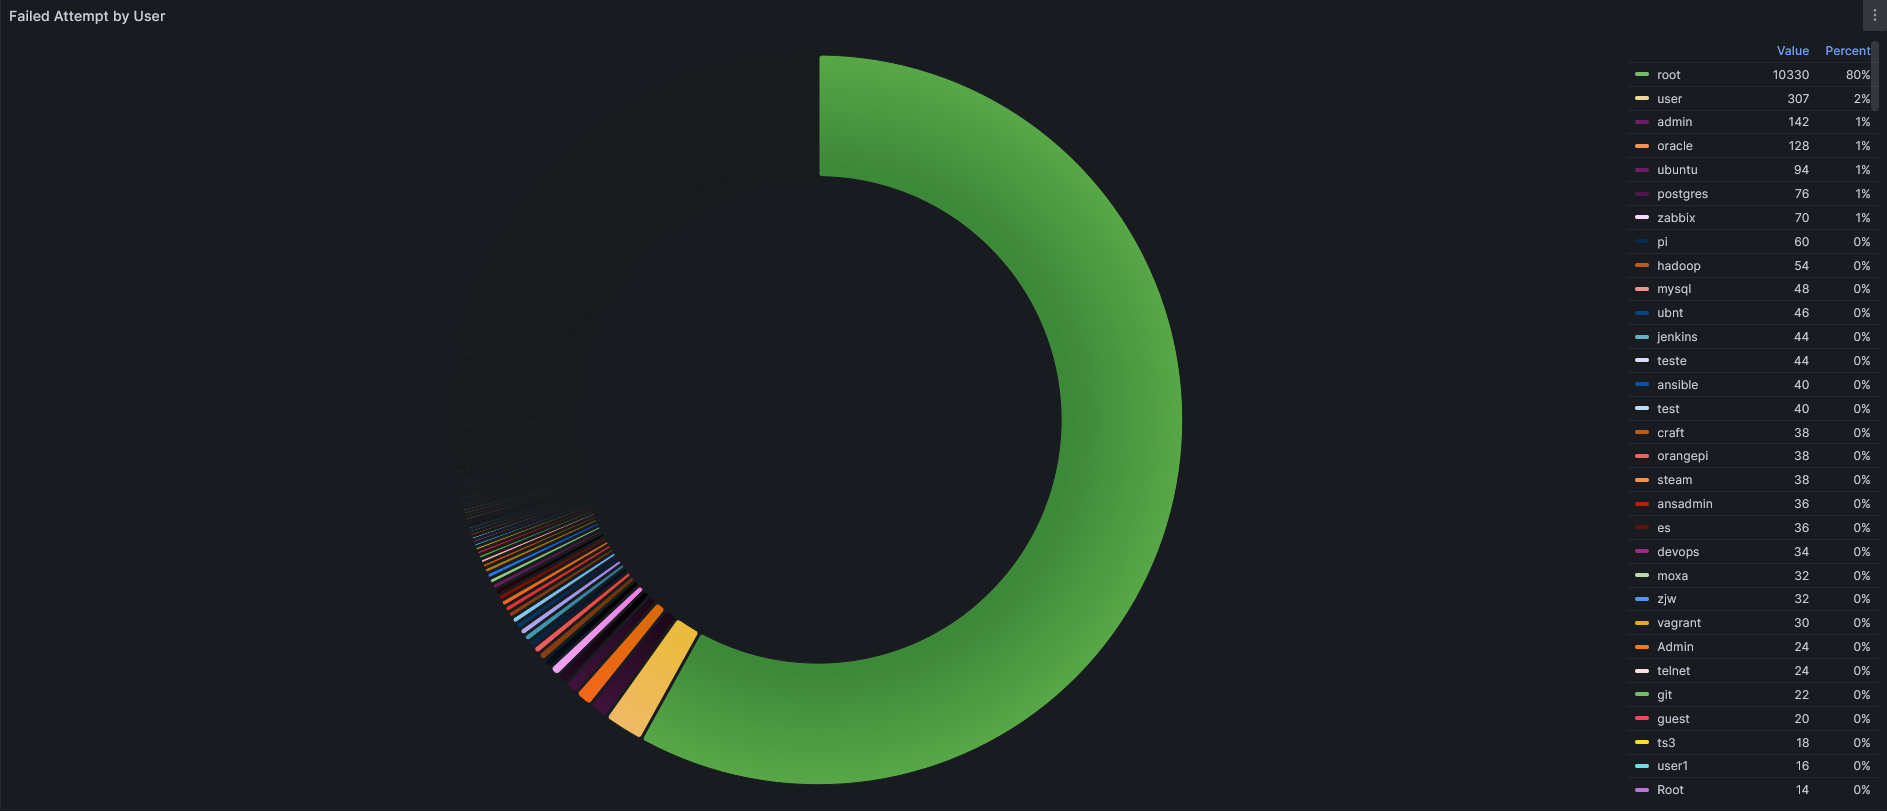
\includegraphics[width=1.7\textwidth]{assets/Failed_pro_user.png}}
        \caption[Kuchendiagramm von Anzahl fehlgeschlagenen Anmeldeversuche pro Benutzername]
        {Kuchendiagramm von Anzahl fehlgeschlagenen Anmeldeversuche pro Benutzername}
        \label{fig:1_Anmeldung_BenutzerName}
        \centering
    \end{figure}
Aus der Abbildung \ref{fig:1_Anmeldung_BenutzerName} können wir ableiten, dass am 22.4.2022 möglicherweise ein \gls{bruteforce} stattfand. Dabei wurden gängige Benutzernamen verwendet, um Anmeldeversuche durchzuführen. Zum Beispiel gab es 10.330 Versuche mit dem Benutzernamen \quotes{root}, 307 Versuche mit \quotes{user} und 142 Versuche mit \quotes{admin}.
\end{landscape}
\restoregeometry

\newpage
\newgeometry{right=30mm, left=30mm}
\thispagestyle{lscape}
\begin{landscape}
  Wir können weitere Filter anwenden, um beispielsweise zu zeigen, zu welchen Uhrzeiten die meisten Versuche stattgefunden haben, wie auf der Graphik \ref{fig:2_Anmeldung_BenutzerName}:
    \begin{figure}[H]
       % \centering
        \centerline{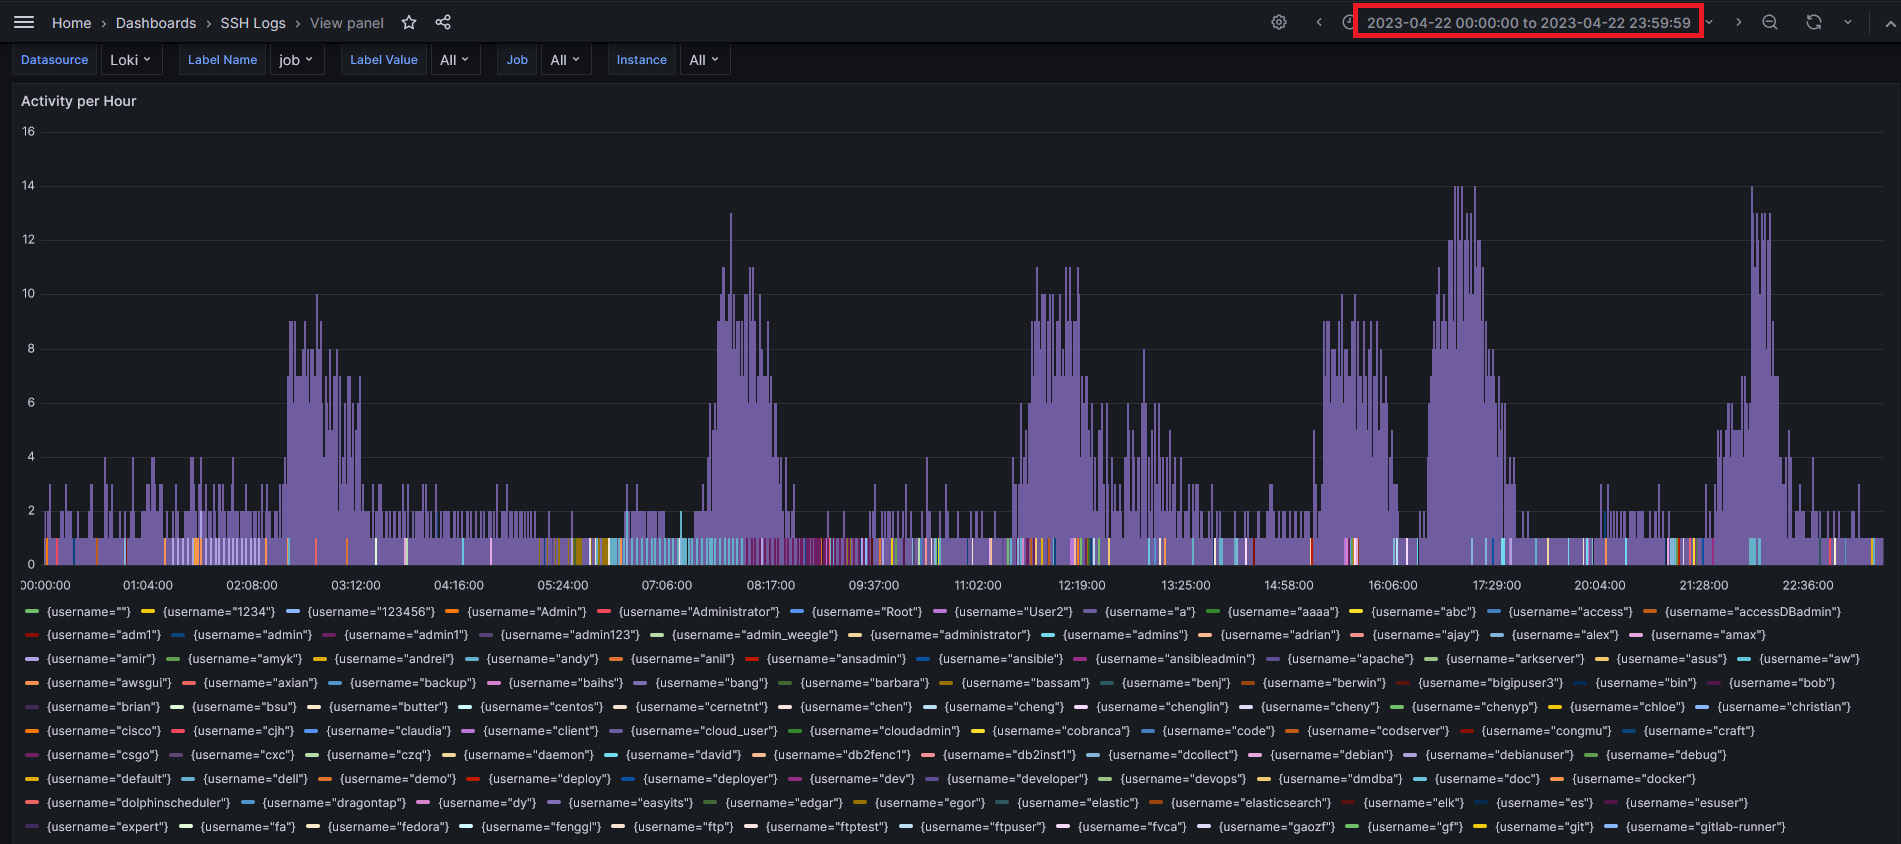
\includegraphics[width=1.5\textwidth]{assets/activityperhour.png}}
        \caption[Balkendiagramm Darstellung der fehlgeschlagenen Anmeldeversuche in einem Zeitfenster von 24 Stunden am \quotes{22.5.2022}]
        {Balkendiagramm Darstellung der fehlgeschlagenen Anmeldeversuche in einem Zeitfenster von 24 Stunden am \quotes{22.5.2022}}
        \label{fig:2_Anmeldung_BenutzerName}
        \centering
    \end{figure}
  Die Abbildung \ref{fig:2_Anmeldung_BenutzerName} zeigt, dass die meisten Versuche zwischen 16:00 und 17:30 Uhr stattfanden.
\end{landscape}
\restoregeometry


Die nächste Abbildung, \ref{fig:1_Anmeldung_IPAdresse}, soll die Anzahl von fehlgeschlagene Anmeldeversuche pro IP-Adresse zeigen. Die benutzten Abfragen lauten wie folgt:
{\setstretch{1.0}
\begin{Verbatim}[frame=single]
count by (ip) (count_over_time({job=~"sshlogs"} 
|="sshd[" 
|~": Invalid
|: Connection closed by authenticating user
|: Failed .* user" 
| pattern `<_> from <ip> port` 
| __error__="" [$__interval]))

count by (ip) (count_over_time({job=~"sshlogs"} 
|="sshd[" 
|=": Failed" !~"invalid user" 
| pattern `<_> from <ip> port` 
| __error__="" [$__interval]))
\end{Verbatim}
}


\newpage
\newgeometry{right=30mm, left=30mm}
\thispagestyle{lscape}
\begin{landscape}
    \begin{figure}[H]
       % \centering
        \centerline{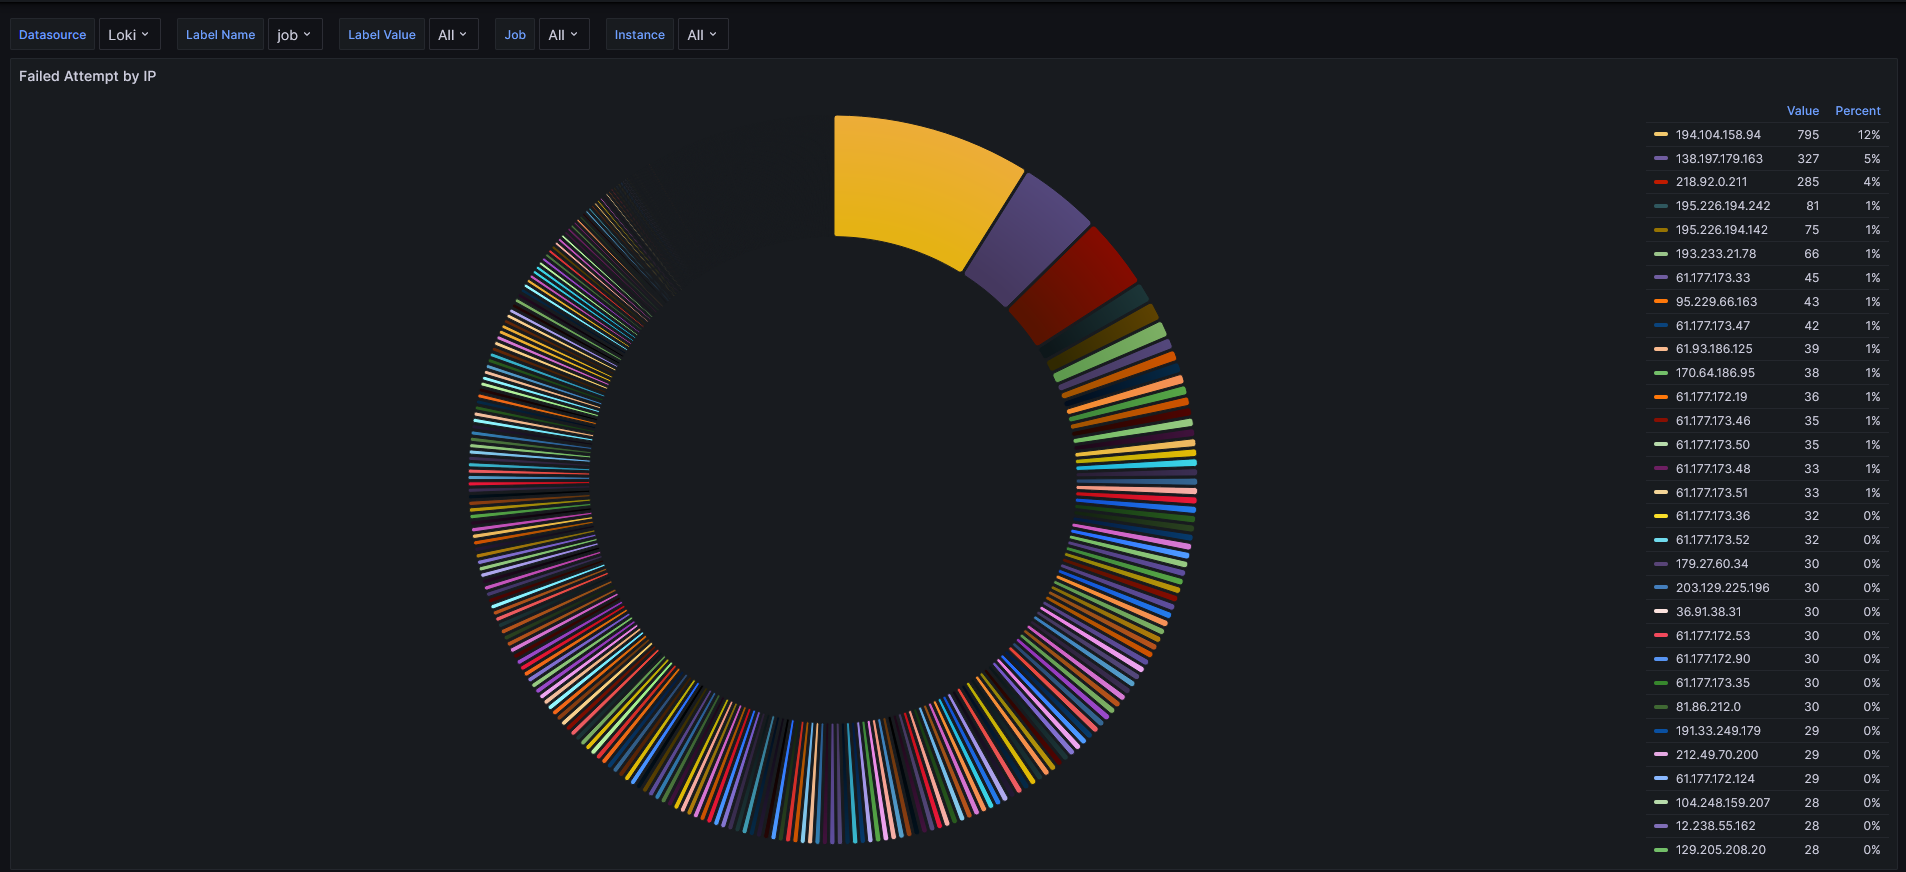
\includegraphics[width=1.6\textwidth]{assets/Failed_pro_ip.png}}
        \caption[Kuchendiagramm von Anzahl fehlgeschlagenen Anmeldeversuche pro IP-Adresse]
        {Kuchendiagramm von Anzahl fehlgeschlagenen Anmeldeversuche pro IP-Adresse}
        \label{fig:1_Anmeldung_IPAdresse}
        \centering
    \end{figure}

Aus Abbildung \ref{fig:1_Anmeldung_IPAdresse} können wir die IP-Adressen identifizieren, von denen die meisten fehlgeschlagenen Anmeldeversuche zwischen dem 21.4.2023 und dem 22.4.2022 stammen.
\end{landscape}
\restoregeometry

\subsection{Generierung von Warnmeldungen}

Mithilfe der oben gezeigten Abfragen generieren wir auch unsere Warnmeldung mit Alerting von Grafana.

Warnmeldungen dienen hauptsächlich der Echtzeitanalyse. Da unsere Logdateien jedoch aus den Monaten März und April 2023 stammen, verschoben wir die Daten in die entsprechenden Monate, um \quotes{Echtzeit}-Daten für die Analyse zu simulieren. Dies ermöglicht uns, aktuelle Warnungen und Alarme basierend auf den verschobenen Daten zu generieren. Wir haben unsere Logdateien so angepasst.

\begin{center}
{\setstretch{1.0}
\begin{Verbatim}[frame=single]
                    Mar ===> Apr | März ====> April
                    Apr ===> May | April ===> May
              26 Apr ===> 27 May | 26 April ===> 27 May
\end{Verbatim}
}
\end{center}

Für unsere Warnmeldung benutzten wir folgende Abfrage:
\begin{center}
{\setstretch{1.0}
\begin{Verbatim}[frame=single]
sum by (Source_IP) (count_over_time({job=~"sshlogs"} 
|="sshd[" 
|~": Invalid
|:Connection closed by authenticating user
|: Failed .* user" 
| pattern `<_> from <Source_IP> port` 
| __error__="" [5m]))
\end{Verbatim}
}
\end{center}

Aus dieser Abfrage finden wir heraus, wie viele fehlgeschlagene Anmeldeversuche pro IP-Adresse es gibt. Mit einem Zeitfenster von einer Woche lösen wir immer dann eine Meldung aus, wenn dieser Wert größer als fünf ist. Fünf ist ein von uns ausgewählter Wert. 

\newpage
In der Abbildung \ref{fig:unsereWarnmeldung1} zeigen wir, wie eine Warnmendung aussieht. wir können auch die Quelladresse des fehlgeschlagenen Anmeldeversuchs erkennen:  
\begin{figure}[H]
  \centering
  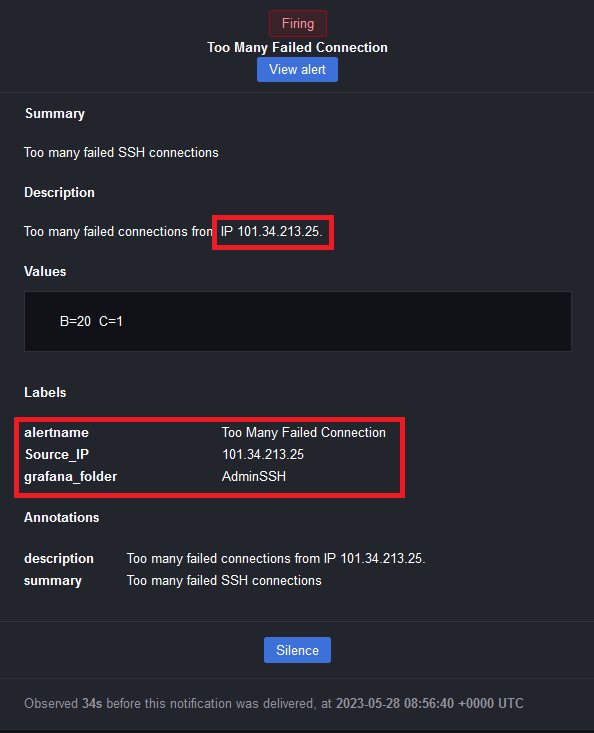
\includegraphics[width=0.6\textwidth]{assets/OurAlert.png}
  \caption[Warnmeldung von Grafana über fehlgeschlagenen \gls{ssh}-Anmeldeversuch]
  {Warnmeldung von Grafana über fehlgeschlagenen \gls{ssh}-Anmeldeversuch}
  \centering
  \label{fig:unsereWarnmeldung1}
\end{figure}

\subsection{Zusammenfassung}

Grafana bietet zahlreiche Möglichkeiten, um Daten zu kombinieren, darzustellen und Warnmeldungen zu generieren. Die Nutzungsmöglichkeiten sind praktisch unbegrenzt und hängen von der Kreativität des Benutzers sowie den Anforderungen der jeweiligen Situation ab.

%Das Alerting Tool von Grafana ist nicht so benutzerfreundlich, wenn es darum geht, die \quotes{labels} in der Nachrichten der Warnmeldung hinzufügen. Obwohl die offiziele Dokumentation ein Beispieldie Nachricht in den Warnmeldungen zu schreiben. 


% unsere Warnmeldung
% unsere Grafik

% fucking alerts

%https://computingforgeeks.com/run-elastic-stack-elk-on-docker/